\begin{frame}
	\frametitle{2-qubit}
	
	\begin{tikzpicture}	
	\node[anchor=south west,inner sep=0] (image) at (0,0) {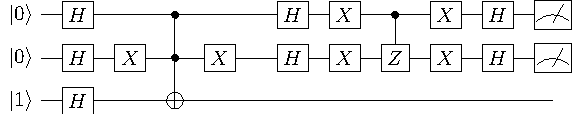
\includegraphics[width=0.9\textwidth]{figures/circuits/2-qubit.pdf}};
	\begin{scope}[x={(image.south east)},y={(image.north west)}]
		%\draw[help lines,xstep=.1,ystep=.1] (0,0) grid (1,1);
		\foreach \x in {0,1,...,9} { \node [anchor=north] at (\x/10,0) {0.\x}; }
		\foreach \y in {0,1,...,9} { \node [anchor=east] at (0,\y/10) {0.\y}; }
		\draw<2->[thick,dashed] (0.085,-0.05) rectangle (0.185,1.05);
		\node<2-> [above] at (0.125,1.1) {Initialization};
	\end{scope}

	\end{tikzpicture}	
\end{frame}